\graphicspath{{3functions/asy/}}


\section{Elementary Functions}\label{chap:functions}

We've already considered polynomials, rational functions and, to some extent, $n\th$ roots and the exponential. We now develop the logarithmic and trigonometric functions.

\subsection[Exponentials \& Logarithms]{Exponential and Logarithmic Functions}% (\S\,30--32, 34)

The exponential function $\exp:\C\to\C:z\mapsto e^z$ was defined earlier using Euler's formula
\[
	\exp(z)=e^z:=e^x\cos y+ie^x\sin y \tag{$\ast$}
\]
For reference, we collect some basic properties: parts 1--3 are identical to real analysis.

\begin{lemm}{}{expbasic}
	Throughout let $z,w\in\C$.
	\begin{enumerate}\itemsep1pt
	  \item The exponential function is entire, with derivative $\diff ze^z=e^z$
	  \item $e^z\neq 0$
	  \item\label{lemmpart:exp4} (Exponential laws)\lstsp $e^{z+w}=e^{z}e^{w}$, \  $e^{z-w}=\frac{e^{z}}{e^{w}}$ and $(e^z)^n=e^{nz}$ (whenever $n\in\Z$).
	  \item\label{lemmpart:exp5} $e^z$ is \emph{periodic} with period $2\pi i$. Moreover,
	  \[
	  	e^z=e^w\iff z-w=2\pi in\text{ for some }n\in\Z
	  \]
	\end{enumerate}
\end{lemm}

\begin{proof}[Sketch Proof]
	\begin{enumerate}\itemsep1pt
	  \item This is Example \ref*{ex:crlots}.\ref{ex:crexex2}: check Cauchy--Riemann and compute $\diff ze^z=u_x+iv_x$.
	  \item This follows trivially from ($\ast$): $e^x>0$ while $\cos y$ and $\sin y$ are never both zero.
	  \item Apply the multiple-angle formulæ for cosine and sine. For the third law, induct with $z=w$.
	  %\item This requires an induction using part 3 with $z=w$.
		\item Certainly $e^{w+2\pi in}=e^w$ by the periodicity of sine and cosine. Now suppose $e^z=e^w$ where $z=x+iy$ and $w=u+iv$. By considering the modulus and argument, we see that
		\[
			e^xe^{iy}=e^ue^{iv}\implies
			\begin{cases}
				e^x=e^u\\
				y=v+2\pi in\text{ for some }n\in\Z
			\end{cases}
		\]
		We conclude that $x=u$ and so $z-w=i(y-v)=2\pi in$.\qedhere
	\end{enumerate}
\end{proof}

\begin{example}{}{}
	Find all $z\in\C$ such that $e^z=5(-1+i)$.\smallbreak
	Following part \ref*{lemmpart:exp5} of the Lemma, write $z=x+iy$ and take the polar form of $5(-1+i)$:
	\begin{align*}
		e^z=5(-1+i)&\iff e^xe^{iy}=5\sqrt 2\polar{3\pi i}4 =e^{\ln(5\sqrt 2)}\polar{3\pi i}4\\
		&\iff
		\begin{cases}
			x=\ln(5\sqrt 2)\\
			y=\frac{3\pi}4+2\pi n\quad\text{ for some }n\in\Z
		\end{cases}\\
		&\iff z=\ln(5\sqrt 2)+\left(\frac{3\pi}4+2\pi n\right)i\quad\text{for some}\quad n\in\Z
	\end{align*}
	We see that there are \emph{infinitely many} suitable $z$!
\end{example}
\goodbreak


\begin{aside}
	\boldinline{Duplicate Notation Warning!}
	
	When $n\in\N$, the expression $e^{\frac 1n}$ could mean two things. For instance $e^{\frac 13}$ might mean either:\smallskip
  \begin{enumerate}\itemsep0pt
    \item The \emph{set} of cube roots of $e$, namely $\{\sqrt[3]{e},\sqrt[3]{e}\polar{2\pi i}3,\sqrt[3]{e}\polarn{2\pi i}3\}$;
    \item The \emph{real value} $\sqrt[3]{e}\in\R^+$.
  \end{enumerate}
  Since $e^z$ is such a common function, we default to the second meaning: if you mean the set of $n\th$ roots, say so! Remember you can always write $\exp(z)$ for the function if necessary.
\end{aside}


The periodicity of the exponential leads to the more subtle notion of the complex \emph{logarithm.}

\begin{defn}{}{log}
	Let $z=re^{i\theta}$ be a non-zero complex number with principal argument $\theta=\Arg z$. The \emph{principal logarithm} of $z$ is the value
	\[
		\Log z:=\ln r+i\theta =\ln\nm z+i\Arg z
	\]
	where $\ln$ is the usual (real!) natural logarithm. The \emph{logarithm} of $z$ is any (and all) of the values\footnotemark
	\[
		\log z=\ln\nm z+i\arg z=\ln r+i(\theta+2\pi n):n\in\Z
	\]
\end{defn}

\footnotetext{%
	This is similar to how $\arg z$ means either the \emph{set} $\{\Arg z+2\pi ni\}$ or some particular value from this set, dependent on context. We'll more formally discuss such \emph{multi-valued} functions in Section \ref{sec:multivalued}.%
}

\begin{examples}{}{}
	\exstart Since $-4=4e^{\pi i}$, we see that
	\[
		\Log(-4)=\ln 4+\pi i\quad\text{and}\quad \log(-4)=\ln 4+(1+2n)\pi i\]
	\begin{enumerate}\setcounter{enumi}{1}
		\item Again write in polar form to compute:
		\[
			\Log(\sqrt 3-i)=\Log(2\polarn{\pi i}6)=\ln 2-\smash{\frac{\pi i}6}\quad\text{and}\quad \log (\sqrt 3-i)=\ln 2-\smash{\frac{\pi i}6}+2\pi ni
		\]
	\end{enumerate}
\end{examples}

These examples involve solving equations of the form $e^w=z$: writing $z=re^{i\theta}=e^{\ln r+i\theta}$ as above, and appealing to part \ref{lemmpart:exp5} of Lemma \ref*{lemm:expbasic}, we instantly see that
\[
	e^w=z\iff w=\log z
\]
Read this carefully, remembering that the logarithm is multi-valued and the exponential periodic:
\[
	e^{\log z}=z
	\quad\text{and}\quad
	\log e^w=w+2\pi ni\quad\text{where $n\in\Z$}
\]
For reference, we summarize some of the basic properties of the principal logarithm function. All parts should be clear from Definition \ref{defn:log}.


\begin{lemm}{}{}
	Throughout, $z$ and $w$ are complex numbers with $z\neq 0$, and $n\in\Z$.
	\begin{itemize}
	  %\item $e^z=w\iff z=\log w$ is \emph{any} logarithm of $w$. That is, $\log(e^z)=z+2\pi in$, for any/all $n$.
	  \item $\Log:\C\setminus\{0\}\to \{w\in\C:-\pi <\Im w\le\pi\}$ is a bijection with inverse $\exp$.
	  \item $\Log e^w=w+2\pi ni$ where $n\in\Z$ is chosen such that $\Im(\Log e^w)=\Im w+2\pi n\in(-\pi,\pi]$.
	  \item If $z\in\R^+$, then $\Log z=\ln z$ is the usual \emph{natural} logarithm.
	\end{itemize}
\end{lemm}


\goodbreak

\boldinline{The Logarithm Laws}\phantomsection\label{sec:loglaws}

Just as the standard rules for exponentiation (Lemma \ref*{lemm:expbasic} part \ref{lemmpart:exp4}) apply to the complex exponential, the log laws also translate. However, the multi-valued nature of the logarithm adds some subtlety.\smallbreak

Suppose non-zero $z,w$ are given: since $\nm{zw}=\nm z\nm w$ and $\arg zw=\arg z+\arg w$, we conclude that
\begin{align*}
	\log zw&=\ln(\nm z\nm w)+i(\arg z+\arg w)\\
	&=\ln\nm z+i\arg z+\ln\nm w+i\arg w\\
	&=\log z+\log w
\end{align*}
Be very careful, for this expression is \emph{not} an identity of \emph{functions.} What it really means is that the following two \emph{sets} are identical:
\begin{gather*}
	\begin{aligned}
		\log z+\log w&=\bigl\{\alpha+\beta:\alpha\in\log z,\beta\in\log w\bigr\}\\
		&=\bigl\{\nm z+i\Arg z+2\pi ki+\nm w+i\Arg w+2\pi mi:k,m\in\Z\bigr\}
		\end{aligned}\\
	\log zw=\bigl\{\ln\nm{zw}+i\Arg(zw)+2\pi ni:n\in\Z\bigr\} 
\end{gather*}
Unless you are sure you won't make a mistake, it is safer to write
\[
	\tcbhighmath{\log zw=\log z+\log w+2\pi ni\quad\text{for some}\quad n\in\Z}
\]
Given its restricted range, we can be more precise for the principal logarithm:
\[
	\tcbhighmath{\Log zw=\Log z+\Log w+2\pi ni\quad\text{for some}\quad n=0,-1,1}
\]


\begin{example}{}{}
	Let $z=-\sqrt 3+i=2\polar{5\pi i}6$ and $w=\sqrt 2(1+i)=2\polar{\pi i}4$. Then, for some $k,m,n$,
  \begin{gather*}
  	\log z=\ln 2+\frac{5\pi i}6 +2\pi ki,\qquad \log w=\ln 2+\frac{\pi i}4+2\pi mi\\
  	\log zw=\log(4e^{\frac{5\pi i}6+\frac{\pi i}4})=\log(4\polar{13\pi i}{12}) =\ln 4+\frac{13\pi i}{12}+2\pi ni
  \end{gather*}
  We can choose particular logarithms satisfying $\log zw=\log z+\log w$ provided $n=k+m$. For principal logarithms, we don't get to make a choice:
  \begin{gather*}
  	\Log z=\ln 2+\frac{5\pi i}6,\qquad \Log w=\ln 2+\frac{\pi i}4\\
  	\begin{aligned}
  		\Log zw&=\Log(4\polarn{11\pi}{12}) =\Log(4\polarn{11\pi}{12}) =\ln 4-\frac{11\pi i}{12}\\
  		&  = \ln 4+ \frac{5\pi i}6+\frac{\pi i}4 -2\pi i
  		=\Log z+\Log w-2\pi i
  	\end{aligned}
  \end{gather*}
\end{example}

We can similarly demonstrate the second log law, with exactly the same caveat:
\[
	\tcbhighmath{\log\frac zw=\log z-\log w}
\]
As before, principal logarithms might require a correction term of $\pm\pi i$.\bigbreak

\vfil
\goodbreak%\clearpage
We can  try to translate the final log law ($\log z^n=n\log z$, $n\in\N$), though even more care is needed!

\begin{example}{}{twolog}
	Let $z=-\sqrt 3+i=2\polar{5\pi i}6$ and compute what is meant by the \emph{set} $2\log z$:
	\[
		2\log z=\left\{2\left(\ln 2+\frac{5\pi i}6 +2\pi mi\right):m\in\Z\right\}
		=\left\{\ln 4+\frac{5\pi i}3+\textcolor{red}{4}\pi mi:m\in\Z\right\}
	\]
	This has only \emph{half} the terms of the set
	\[
		\log z^2=\left\{\log(4\polar{10\pi i}6)=\ln 4+\frac{5\pi i}3+\textcolor{blue}{2}\pi ki :k\in\Z\right\}
	\]
	It is therefore safer to state that $\log z^2\neq 2\log z$.
\end{example}

Since the principal logarithm is a function rather than a set, we can be more precise: for any $n\in\N$,
\[
	\tcbhighmath{\Log z^n=n\Log z+2\pi ki
	\quad\text{for some integer $k$ with}\ \nm k\le \frac n2}
\]

\begin{example}{}{}
	Let $z=\polarn{13\pi i}{16}$ and consider $z^{16}$. We see that
	\[
		\Log z^{16}=\Log e^{-13\pi i}=\Log e^{\pi i} =i\pi,
		\quad 16\Log z=-13\pi i
		\implies \Log z^{16}=16\Log z+14\pi i
	\]
	In this case $\nm k=7\le \frac{16}2$.
\end{example}


\begin{exercises}
	\exstart Compute (be careful with (c)!):
	\begin{enumerate}\setcounter{enumi}{1}
	  \item[]\begin{enumerate}
	  	\item\ $\exp(3-\frac\pi 2 i)$\qquad
	  	(b) \ $\Log(ie)$\qquad
	  	(c) \ $\log(3-4i)$\qquad
	  	(d) \ $\Log[(-1+i)^2]$
	  \end{enumerate}
  
	  \item\begin{enumerate}
	    \item If $e^z$ is real, show that $\Im z=n\pi$ for some integer $n$.
	    %\item If $e^z$ is a \emph{negative} real number, what can we say about $z$?
	    \item If $e^z$ is imaginary, what restriction is placed on $z$?
	  \end{enumerate}
	  
	  \item Show in two ways that the function $f(z)=\exp(z^2)$ is entire, and find its derivative.
	  
	  \item Prove, for any $z\in\C$, that $\nm{\exp(z^2)}\le \exp\nm z^2$. What must $z$ satisfy if this is to be \emph{equality}?
	  
	  \item Find $\Re e^{\frac 1z}$ in terms of $x$ and $y$. Why is $\Re e^{\frac 1z}$ harmonic on any domain not containing the origin?
	  
	  \item Show that $\Log i^3\neq 3\Log i$.
	  
	  \item Show that $\Re(\log (z-1))=\frac 12\ln[(x-1)^2+y^2]$ whenever $z\neq 1$.
	  
	  \item Prove the above boxed formula for $\Log z^n$.
	  
	  \item The square roots of $i$ are $\sqrt i=\polar{\pi i}4$ and $-\sqrt i=\polarn{3\pi i}4$.
	  \begin{enumerate}
	    \item Compute $\Log\sqrt i$ and $\Log(-\sqrt i)$ and check that $\Log\sqrt i=\frac 12\Log i$.
	    \item Show that the set of all logarithms of all square roots of $i$ is
	    \[
	    	\log i^{\frac 12}=\left(n+\frac 14\right)\pi i\quad\text{where}\quad n\in\Z
	    \]
	    Hence deduce that $\log i^{\frac 12}=\frac 12\log i$ \emph{as sets.}
			%\item Can you relate the principal logarithms of the two square roots of $i$?
		\end{enumerate}
	\end{enumerate}
\end{exercises}

\goodbreak



\subsection[Multi-valued Functions]{Multi-valued Functions, Branch Cuts and the Power Function}\label{sec:multivalued}%(\S\,33, 35, 36)

Recall that each $\log z$ represents a set of complex numbers; as such, the complex logarithm is termed a \emph{multi-valued function.} We have previously encountered others of this ilk:
\begin{itemize}
  \item The \emph{argument} of a complex number is any of the values $\arg z=\Arg z+2\pi n$ where $n\in\Z$. The complex logarithm is merely a modification of this: $\log z=\ln\nm z+i\arg z$.
  \item The \emph{$n\th$ root} of $z$ is the set of values $z^{\frac 1n}=\{\sqrt[n]{z}\omega_n^k:k=0,\ldots,n-1\}$ where $\omega_n=\polar{2\pi i}n$ is an $n\th$ root of unity and $\sqrt[n]{z}$ the principal $n\th$ root.
\end{itemize}
It is an abuse of language to refer to a multi-valued \emph{function,} since any function should assign \emph{exactly one} output to each element of its domain. While this problem can be fixed using equivalence classes, another approach is simpler to visualize.

\begin{defn}{}{}
	A \emph{branch} of a multi-valued function $f$ is a single-valued function $F$ on a domain $D$ which is \emph{holomorphic} (differentiable) on $D$ and such that each $F(z)$ is one of the values of $f(z)$.\smallbreak
	Let $D=\C\setminus\ell$ where $\ell$ is a line or curve in $\C$. If $F:D\to\C$ is a branch of $f$, we call $\ell$ a \emph{branch cut.} A \emph{branch point} is any point common to all possible branch cuts.
\end{defn}

\begin{minipage}[t]{0.7\linewidth}\vspace{0pt}
\boldinline{Branches of the Logarithm}
	The \emph{principal branch} of the logarithm is a slightly restricted version of the principal logarithm
	\[
		\Log z=\ln r+i\theta\ \text{ where }\ \theta=\Arg z\in(-\pi,\pi)
	\]
	The branch cut is the non-positive real axis. To check holomorphicity, we verify the Cauchy--Riemann equations:\footnotemark
	\[
		ru_r=r\partials{r}\ln r=1=\partials{\theta}\theta=v_\theta
		,\qquad
		u_\theta=0=-rv_r
	\]
	The partial derivatives are certainly continuous, whence $\log z$ is holomorphic with derivative 
	\[
		\diff z\log z=e^{-i\theta}(u_r+iv_r)=\frac 1re^{-i\theta}=\frac 1z
	\]
	More generally, for any angle $\alpha$ we could take a branch cut $\ell$ to be the line with argument $\alpha$, which defines a new branch of the logarithm:
	\[
		\log z=\ln r+i\theta
		\ \text{ where }\
		\theta\in (\alpha-2\pi,\alpha)
	\]
	In this description, the principal branch corresponds to $\alpha=\pi$. Note that choosing $\alpha=-\pi$ results in the \emph{same branch cut}, but a \emph{different branch}:
\end{minipage}
\hfill
\begin{minipage}[t]{0.29\linewidth}\vspace{0pt}
	\flushright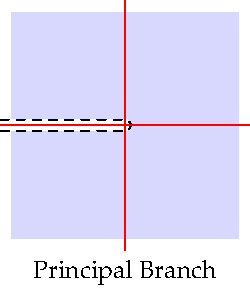
\includegraphics{branch1}
	\medbreak
	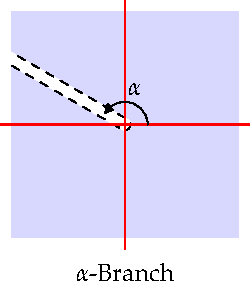
\includegraphics{branch2}
\end{minipage}
\[
	\log z=\ln r+i\theta\ \text{ where }\ \theta\in(-3\pi,-\pi)
\]


\footnotetext{%
	We use the polar form: $ru_r=v_\theta$, $rv_r=-u_\theta$, $f'(z)=e^{-i\theta}(u_r+iv_r)$ (see Exercise \ref*{subsec:analytic}.\ref{exs:crpolar}).
}

\goodbreak

\begin{minipage}[t]{0.72\linewidth}\vspace{0pt}
	More esoteric branch cuts are possible, such as the pictured `squiggle.' At issue is the fact that traversing a \textcolor{Green}{counter-clockwise loop around the origin} increases the value of a logarithm  by $2\pi i$. It is therefore impossible for a branch to be \emph{continuous} (let along \emph{holomorphic}) on any domain containing such a \textcolor{Green}{loop}; to make $\log z$ single-valued, a branch cut must `cut' any such \textcolor{Green}{path}, and thus connect the two \emph{branch points} 0 and $\infty$.\smallbreak
	Clarity is crucial here: when you write $\log z$, do you mean a \emph{set,} a particular \emph{element} of that set, or a \emph{branch}? Certain expressions may be true or false depending on the meaning.
\end{minipage}
\hfill
\begin{minipage}[t]{0.27\linewidth}\vspace{0pt}
	\flushright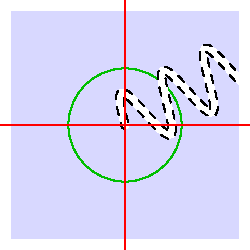
\includegraphics{branch3}
\end{minipage}



\begin{example}{}{}
	Consider $z=\frac 1{\sqrt 2}(1+i)=\polar{\pi i}4$. For the principal branch, we have
	\[
		\Log z^2=\Log \polar{\pi i}2 =\frac{\pi i}2 =2\Log z
	\]
	For the branch with $\alpha=\frac{\pi}3$ (that is, $\arg z\in(\frac{-5\pi}3,\frac{\pi}3)$), we have
	\[
		z^2=\polar{\pi i}2=\polarn{3\pi i}2\implies \log z^2=-\frac{3\pi i}2 \neq 2\log z
	\]
	Recall also (Example \ref{ex:twolog}), that \emph{as sets,} $\log z^2\neq 2\log z$. 
\end{example}

For individual branches of the logarithm, specific versions of the logarithm laws (page \pageref{sec:loglaws}) are available, though they are not worth trying to remember; just carefully think out the possibilities when calculating.



\boldinline{General Exponential Functions}

The logarithm can be used to create exponential functions for any non-zero complex base $c$. Choose a value $\log c$ and define
\[
	\tcbhighmath{c^z:=e^{z\log c}}
\]
Provided $c$ is not a non-positive real number, the standard is to use the principal logarithm. Regardless of your choice, $\log c$ is constant and the exponential function is holomorphic everywhere:
\[
	\diff zc^z=c^z\log c
\]

\begin{example}{}{expifunc}
	Let $c=i=\polar{\pi i}2$ and use the principal logarithm to define
	\[
		i^z:=e^{z\Log i}=\exp\left(\frac{\pi iz}2\right) =\exp\left(-\frac\pi 2y+i\frac\pi 2x\right) =\polarn{\pi y}2\left[\cos\frac\pi 2x+i\sin\frac\pi 2x\right]
	\]
	It is simple to check the Cauchy--Riemann equations and see that $i^z$ is entire (holomorphic on $\C$).\smallbreak
	If we instead took a different branch of the logarithm with $\arg i=-\frac{3\pi i}2$, then
	\[
		i^z=\exp\left(\frac{-3\pi iz}2\right) =\polar{3\pi y}2\left[\cos\frac{3\pi}2x-i\sin\frac{3\pi}2x\right]
	\]
	This is still entire, though it is a completely different function! Note that both choices of $i^z$ agree whenever $z$ is an integer, and for $z=\frac 12$ they produce the two distinct square roots of $i$!
\end{example}

\goodbreak



\boldinline{Power Functions}

Following a similar approach, for any non-zero $z$ and complex number $c$ we may define the (typically multi-valued) function
\[
	\tcbhighmath{z^c:=e^{c\log z}}
\]
In this case, restricting to the principal branch of the logarithm gives an unambiguous function.

\begin{defn}{}{}
	The \emph{principal value} of $z^c$ is the function
	\[
		\operatorname{P.V.}z^c:=e^{c\Log z}
	\]
	whose domain is that of the logarithm ($\C$ excluding the non-positive real axis).
\end{defn}



\begin{example}{}{}
	Using the principal branch of the logarithm ($\Theta=\Arg z$), we obtain
	\[
		\operatorname{P.V.}z^{\frac 13}=\exp\left(\frac 13(\ln r+i\Theta)\right) =\exp\left(\ln \sqrt[3]{r}+\frac{i\Theta}3\right)=\sqrt[3]{r}\polar{i\Theta}3 =\sqrt[3]{z}
	\]
	precisely the principal cube-root of $z$ as defined previously.\smallbreak
	If we chose a different branch with $\arg z=\theta$, then
	\[
		z^{\frac 13} =e^{\frac 13\log z}=\exp\left(\frac 13(\ln r+i\theta)\right) =\sqrt[3]{r}\exp\left(\frac i3(\Theta+(\theta-\Theta))\right) =\sqrt[3]{z}\polar{i(\theta-\Theta)}3
	\]
	Since, for any $z$, the difference in the arguments $\theta-\Theta=2\pi n$ is a multiple of $2\pi$, this expression really does return one of the cube-roots of $z$.
\end{example}

\begin{lemm}{}{}
	Choose a branch of the logarithm so that $z^c=e^{c\log z}$ is single-valued. Then $z^c$ is holomorphic on the same domain as the logarithm; moreover $\diff zz^c=cz^{c-1}$.
\end{lemm}

\begin{proof}
	Since $\log z$ is holomorphic, simply use the chain rule:
	\[
		\diff zz^c=\diff ze^{c\log z}=e^{c\log z}\diff z(c\log z)=e^{c\log z}\cdot\frac cz =ce^{c\log z}e^{-\log z}=ce^{(c-1)\log z}=cz^{c-1}\tag*{\qedhere}
	\]
\end{proof}

\begin{example}{}{}
	If the principal branch of the logarithm is used, then
  \[
  	(zw)^c=\exp(c\Log(zw))=\exp(c\Log z+c\Log w+2\pi cn i)=z^cw^ce^{2\pi cn i}
  \]
  for some $n\in\{0,\pm 1\}$. \emph{We do not expect} simple exponent rules such as $(ab)^c=a^cb^c$ to hold in complex analysis! Note, however, that this does work in the case where $c$ is an integer.\smallbreak
  As an example, again using principal values, if $z=w=\polar{3\pi i}4$, then $zw=\polar{3\pi i}2=\polarn{\pi i}2$, whence
  \begin{gather*}
  	\operatorname{P.V.}(zw)^{5i}=\exp\left(5i\cdot \frac{-\pi i}2\right) =\polar{5\pi}2\\
  	\operatorname{P.V.}z^{5i}=\operatorname{P.V.}w^{5i}=\exp\left(5i\cdot \frac{3\pi i}4\right) =\polarn{15\pi}4\\
  	\implies (zw)^{5i} =\polar{5\pi}2 = \polarn{15\pi}2e^{10\pi} =z^{5i}w^{5i} e^{2\pi\cdot 5i\cdot ni}\ \text{ with } \ n=-1
  \end{gather*}
\end{example}



\begin{exercises}
	\exstart Show that the function $f(z)=\Log(z-i)$ is holomorphic everywhere except on the portion $x\le 0$ of the line $y=1$.
	\begin{enumerate}\setcounter{enumi}{1}
  	\item Show that the function $f(z)=\frac 1{z^2+i}\Log(z+4)$ is holomorphic everywhere except at the points $\pm\frac 1{\sqrt 2(1-i)}$ and on the portion $x\le -4$ of the real axis.

  
  	\item Show that the set $z^{\frac 14}$ as defined earlier in the course coincides with the set $z^{\frac 14}:=\exp\left(\frac 14\log z\right)$ as defined in this section.
  
  	\item Show that $(1+i)^i=\exp\left(-\frac \pi 4+2n\pi\right)\exp\left(i\frac{\ln 2}2\right)$ where $n\in\Z$.
  
	  \item Find the principal values of the following:
	  \begin{enumerate}
	  	\item $i^{2i}$\qquad
	  	(b) \ $(1-i)^{3i}$\qquad
	  	(c) \ $(-\sqrt 3+i)^{1+4\pi i}$
	  \end{enumerate}
  
  
  	\item Suppose $c,c_1,c_2$ and $z$ are complex numbers where $z\neq 0$. If all the powers involved are principal values, show that,
	  \begin{enumerate}
	  	\item $z^{c_1}z^{c_2}=z^{c_1+c_2}$\qquad
	  	(b) \ $(z^c)^n=z^{cn}$ for any $n\in\N$.
	  \end{enumerate}
	  
	  \item The power function $z^c$ is \emph{usually} multi-valued. However, if $c=m$ is an integer, prove that $z^m$ is single-valued: i.e.\ it is independent of the branch of logarithm used in its definition.
	  
	  \item Check the claim at the bottom of Example \ref{ex:expifunc}: if $m\in\Z$, then $i^m$ is the same value for the two definitions of $i^z$.
	  
	  \item Continuing the previous question, suppose $c\neq 0$ and define $c^z=e^{z\log c}$ where any choice of the branch of the logarithm is made.
	  \begin{enumerate}
	    \item Let $m\in\Z$. Prove that $c^m$ produces the same value, regardless of the branch of logarithm used to define $\log c$.
	    \item If $z=\frac 1m$, show that $c^z$ really is an $m^\text{th}$ root of $c$. If the principal branch of the logarithm is used, show that $c^z$ is the principal $m^\text{th}$ root of $c$. For every $m^\text{th}$ root of $c$, show that there exists a branch of the logarithm for which $c^z$ equals the given $m^\text{th}$ root.
	  \end{enumerate}
	   
	\end{enumerate}
\end{exercises}
\clearpage




\subsection[Trigonometric Functions]{Trigonometric and Inverse Trigonometric Functions}%(\S\,37--40)

A sensible definition of the basic trigonometric functions comes simply by modifying Euler's formula. For instance, if $y\in\R$, then
\[
	e^{iy}+e^{-iy}=\cos y+i\sin y+\cos y-i\sin y=2\cos y
\]
This motivates the primary definition.

\begin{defn}{}{}
	For any $z\in\C$ we define
	\[
		\cos z=\frac{e^{iz}+e^{-iz}}2
		\qquad
		\sin z=\frac{e^{iz}-e^{-iz}}{2i}
	\]
\end{defn}

\begin{example}{}{cossimple}
	$\cos(\frac\pi 4+i)=\frac 12\bigl(e^{\frac{i\pi}4-1}+e^{\frac{-i\pi}4+1}\bigr)=\frac 12\left(\frac{e^{-1}}{\sqrt 2}(1+i)+\frac{e}{\sqrt 2}(1-i)\right) =\frac{e+e^{-1}}{2\sqrt 2}-\frac{e-e^{-1}}{2\sqrt 2}i$
\end{example}

\begin{thm}{}{}
	Sine and cosine are entire with the same derivatives are their real counterparts
	\[
		\diff z\sin z=\cos z\qquad \diff z\cos z=-\sin z
	\]
	The usual identities, including double and multiple-angle formulæ, are satisfied: for instance
	\[
		\sin^2\!z+\cos^2\!z=1,\quad \cos(z+w)=\cos z\cos w-\sin z\sin w,\quad \cos 2z=2\cos^2\!z-1,\quad\text{etc.}
	\]
	In particular, $\sin z=\cos(z-\frac \pi 2)$ and $\cos z=\sin(z+\frac\pi 2)$. Sine and cosine are also $2\pi$-periodic and have exactly the same zeros as their real versions:
	\[
		\sin z=0\iff z=n\pi,\quad \cos z=0\iff z=\frac\pi 2+n\pi
		\quad\text{where}\quad
		n\in\Z
	\]
\end{thm}

The upshot of the Theorem is that sine and cosine behave exactly as you'd expect.\smallbreak

The proofs are straightforward applications of properties of the exponential function. For instance;
\[
	\diff z\sin z = \diff z\frac{e^{iz}-e^{-iz}}{2i} =\frac 1{2i}(ie^{iz}+ie^{-iz}) =\cos z
\]
and,
\[
	\sin z=0\iff e^{iz}=e^{-iz}\iff e^{2iz}=1\iff e^{-2y}(\cos 2x+i\sin 2x)=1\iff z=\pi n
\]


The remaining trigonometric functions are defined in the expected way: e.g.,
\[
	\tan z=\frac{\sin z}{\cos z}=\frac{e^{iz}-e^{-iz}}{i(e^{iz}+e^{-iz})}
	\quad\text{whenever}\quad
	z\neq \frac\pi 2+n\pi
\]
All trigonometric functions are holomorphic wherever defined and have the usual expressions for their derivatives: e.g., by the quotient rule,
\[
	\diff z\tan z =\diff z\frac{\sin z}{\cos z} =\frac{\cos^2\!z+\sin^2\!z}{\cos^2\!z}=\sec^2\!z
\]

\begin{aside}
	\boldinline{Aside: Hyperbolic Functions}
	
	By considering real and imaginary parts, 
	\begin{align*}
		\sin z&=\frac 1{2i}(e^{ix-y}-e^{-ix+y})=\frac 1{2i}(e^{-y}\cos x+ie^{-y}\sin x-e^y\cos x+ie^y\sin x)\\
		&=\frac 12(e^y+e^{-y})\sin x+\frac i2(e^y-e^{-y})\cos x = \sin x\cosh y+i\cos x\sinh y\\
		\cos z&=\cos x\cosh y-i\sin x\sinh y
	\end{align*}
	where $\cosh y=\frac 12(e^y+e^{-y})$ and $\sinh y=\frac 12(e^y-e^{-y})$ are the usual (real) hyperbolic functions. We could have written Example \ref{ex:cossimple} this way
	\[
		\cos\left(\frac\pi 4+i\right) =\frac{e+e^{-1}}{2\sqrt 2}-i\frac{e-e^{-1}}{2\sqrt 2} =\cos\frac\pi 4\cosh 1-i\sin\frac\pi 4\sinh 1
	\]
	Hyperbolic functions are a convenient short-cut, but never necessary; use or ignore as you like. All their properties can be derived from their relationship to exponential and trigonometric functions:
	\[
		\cosh z=\frac{e^z+e^{-z}}2=\cos iz,\qquad \sinh z=\frac{e^z-e^{-z}}2=-i\sin iz
	\]
	For instance
	\begin{gather*}
		\diff z\sinh z=-i\diff z\sin iz=-i^2\cos iz=\cosh z
		\quad\text{and}\quad
		\diff z\cosh z=\sinh z\\
		\cosh^2\!z-\sinh^2\!z=\cos^2 (iz)+\sin^2 (iz)=1
	\end{gather*}
\end{aside}


\boldinline{Inverse Trigonometric Functions}

As with logarithms, inverting trigonometric functions results in multi-valued functions.

\begin{example}{}{invcos}
	We find an expression for $\cos^{-1}z$ and compute its derivative.
	\[
		w=\cos^{-1}z\iff z=\cos w\iff 2z=e^{iw}+e^{-iw}\iff (e^{iw})^2-2ze^{iw}+1=0
	\]
	which is quadratic in $e^{iw}$. Apply the quadratic formula to see that
	\[
		e^{iw}=\frac{2z+(4z^2-4)^{\frac 12}}2=z+i(1-z^2)^{\frac 12} \iff \cos^{-1}z=w=-i\log\left[z+i(1-z^2)^{\frac 12}\right]
	\]
	A branch of $\cos^{-1}$ requires us to choose branches of \emph{both} the square-root \emph{and} the logarithm.\smallbreak
	Inverse cosine is holomorphic since it is a composition of holomorphic functions. By the chain rule,
	\begin{align*}
		\diff z\cos^{-1}z&=\frac{-i}{z+i(1-z^2)^{\frac 12}}\diff z\left[z+i(1-z^2)^{\frac 12}\right] =\frac{-i}{z+i(1-z^2)^{\frac 12}}\left[1-\frac{iz}{(1-z^2)^{\frac 12}}\right]\\
		&=\frac{-i}{z+i(1-z^2)^{\frac 12}}\cdot\frac{(1-z^2)^{\frac 12}-iz}{(1-z^2)^{\frac 12}} =\frac{-1}{(1-z^2)^{\frac 12}}
	\end{align*}
	If we fix a branch of the square-root (and logarithm) so that $\cos^{-1}z$ is single-valued, this is necessarily the same branch that appears in the expression of the derivative. 
\end{example}

\goodbreak


Expressions such as these are not worth memorizing; they are not difficult to derive when needed using the method in Example \ref{ex:invcos}. Here is the complete list for the three basic functions.


\begin{thm}{}{invtrig}
	The inverse sine, cosine and tangent functions are given by the expressions
	\begin{gather*}
		\sin^{-1}z = -i\log\left[iz+(1-z^2)^{\frac 12}\right] \quad
		\cos^{-1}z=-i\log\left[z+i(1-z^2)^{\frac 12}\right] \quad
		\tan^{-1}z=\frac i2\log\frac{i+z}{i-z}
	\end{gather*}
	Once branches of the square-root (sine/cosine only) and logarithm are chosen, these are holomorphic on their domains and have familiar derivatives:
	\[
		\diff z\sin^{-1}z=\frac 1{(1-z^2)^{\frac 12}}\qquad \diff z\cos^{-1}z=\frac{-1}{(1-z^2)^{\frac 12}}\qquad \diff z\tan^{-1}z=\frac 1{1+z^2}
	\]
	The branches of the square-root in the derivatives of inverse sine and cosine are identical to those used in the definitions of the original functions.
\end{thm}


\begin{examples}{}{}
	\exstart To evaluate $\sin^{-1}\frac 1{\sqrt 2}$ as a complex number, we could follow the approach of Example \ref{ex:invcos} (solve $\frac{e^{iz}-e^{-iz}}{2i}=\frac 1{\sqrt 2}$ directly), or use the formula in Theorem \ref{thm:invtrig}:
  \[
  	\sin^{-1}\frac 1{\sqrt 2} =-i\log\left[\frac i{\sqrt 2}\pm \sqrt{1-\frac 12}\right] =-i\log\frac{i\pm 1}{\sqrt 2}
  \]
  Now evaluate the logarithms separately:
  \begin{gather*}
	  -i\log\frac{i+1}{\sqrt 2} =-i\log \polar{\pi i}4 =-i\left[\frac{\pi i}4+2\pi ni\right] =\frac\pi 4+2\pi n\\
	  -i\log\frac{i-1}{\sqrt 2} =-i\log\polar{3\pi i}4 =-i\left[\frac{3\pi i}4+2\pi ni\right] =\frac{3\pi}4+2\pi n
  \end{gather*}
  The set of values $\sin^{-1}\frac 1{\sqrt 2}$ generated by all branches of the square-root and logarithm is precisely the set we'd have found working entirely within $\R$!
  
	\begin{enumerate}\setcounter{enumi}{1}
	  \item We can also evaluate inverse sines that would have no meaning in $\R$. For instance,
	  \begin{align*}
	  	\sin^{-1}7&=-i\log[7i\pm\sqrt{-48}] =-i\log(7\pm 4\sqrt 3)i =-i\log (7\pm 4\sqrt 3)\polar{\pi i}2\\
	  	&=-i\left[\ln(7\pm 4\sqrt 3)+\frac{\pi i}2+2\pi ni\right] =-i\ln(7\pm 4\sqrt 3)+\frac\pi 2+2\pi n
	  \end{align*}
	  Note that $7>4\sqrt 3$, so we are always taking natural log of a positive real number!
	  
	  \item\label{ex:taninv} Compute $\tan^{-1}(i-2\sqrt 3)$. First compute the required fraction in polar form:
	  \[
	  	\frac{i+(i-2\sqrt 3)}{i-(i-2\sqrt 3)} =\frac{2i-2\sqrt 3}{2\sqrt 3}=-1+\frac i{\sqrt 3}=\frac 2{\sqrt 3}\polar{5\pi i}6
	  \]
	  It follows that
	  \[
	  	\tan^{-1}(i-2\sqrt 3)=\frac i2\left(\ln\frac 2{\sqrt 3}+\frac{5\pi}6i-2\pi ni\right) =-\frac{5\pi}{12}+\frac i2\ln\frac 2{\sqrt 3}+\pi n:\quad n\in\Z
	  \]
	  Choosing the principal value of the logarithm ($n=0$) yields $-\frac{5\pi}{12}+\frac i2\ln\frac 2{\sqrt 3}$.
	\end{enumerate}
\end{examples}
  

\begin{exercises}
	\exstart Find the real and imaginary parts of $\sin i$, $\cos(1+i)$ and $\tan(2i\ln 5+\frac\pi 2)$.
	
	\begin{enumerate}\setcounter{enumi}{1}
	  \item As a sanity check, if $w =-i\log\left[z+(z^2-1)^{\frac 12}\right]$, compute $\cos w=\frac 12(e^{iw}+e^{-iw})$ directly and verify that you obtain $z$, \emph{irrespective} of which branches are chosen.
	  
	  
	  \item Using the real and imaginary parts of $\sin z$, directly verify that the Cauchy--Riemann equations are satisfied.
	  
	  
	  \item Prove the following double/multiple-angle formulæ using the definitions in this section:
	  \begin{enumerate}
	    \item $\cos 2z=2\cos^2z-1$
	    \item $\sin(z-w)=\sin z\cos w-\cos z\sin w$
	    \item $\tan(z+w)=\dfrac{\tan z +\tan z}{1-\tan z\tan w}$
	  \end{enumerate}
	  
	  
	  \item Find all the values of $\tan^{-1}(1+i)$.
	  
	  
	  \item Solve the equation $\cos z=\sqrt 2$ for $z$.
	  
	  
	  \item\label{ex:tanhint} Recall Exercise \ref{ex:taninv}: check explicitly that $\tan w=i-2\sqrt 3$ when $w=-\frac{5\pi}{12}+\frac i2\ln\frac 2{\sqrt 3}$.\par
	  (\emph{Hint: use $\tan w=\frac{e^{2iw}-1}{i(e^{2iw}+1)}$. Why is this true?})
	  
	  
	  \item Suppose $z>1$ is real. Prove that $\Re\sin^{-1}z=\frac\pi 2+2\pi n$ is independent of $z$. What is $\Im\sin^{-1}z$.
	  
	  
	  \item If the same branch of square-root is chosen in each case, prove that $\sin^{-1}z+\cos^{-1}z$ is constant.
	  
	  
	  \item Derive the expressions for $\tan^{-1}z$ and its derivative in Theorem \ref{thm:invtrig}.
	  
	  
	  \item\begin{enumerate}
	    \item Given $\cosh z=\cos(-iz)$, find an expression in terms of the complex logarithm for $\cosh^{-1}z$.
	    \item Using your answer to part (a), or otherwise, find all solutions to the equation $\cosh z=\sqrt 3$.
	    \item Find an expression for the derivative of $\cosh^{-1}z$.
	  \end{enumerate} 
	\end{enumerate}
\end{exercises}